% !Rnw weave = Sweave
\documentclass[10pt,a4paper]{report}
\usepackage{Sweave} 
\usepackage{natbib}
\usepackage{graphics}
\usepackage{amsmath}
\usepackage{indentfirst}
\usepackage{hanging}
%\usepackage{zi4}
%\usepackage[utf8]{inputenc}
\usepackage{hyperref}
\usepackage[T1]{fontenc}
\DeclareGraphicsExtensions{.png,.pdf,.jpg}

\begin{document}

%\VignetteIndexEntry{Species distribution modeling with three-step pseudo--absences}
%\VignetteDepends{mopa,sp,raster,earth}
%\VignetteKeyword{spatial}

%\newcommand{\super}[1]{\ensuremath{^{\textrm{#1}}}}
%\newcommand{\sub}[1]{\ensuremath{_{\textrm{#1}}}}
%\newcommand{\R}{{\normalfont\textsf{R }}{}}









\Sconcordance{concordance:mopa.tex:mopa.Rnw:%
1 60 1 1 2 1 0 3 1 1 4 7 0 1 2 4 1 1 3 2 0 1 1 4 0 1 2 6 1 1 2 1 0 4 1 %
3 0 1 2 2 1 1 2 4 0 1 2 3 1 1 2 1 0 1 1 1 3 6 0 1 2 6 1 1 4 3 0 2 1 4 0 %
1 2 5 1 1 4 9 0 4 1 4 0 1 2 4 1 1 5 9 0 3 1 5 0 1 3 2 1 1 5 9 0 3 1 4 0 %
1 2 2 1 1 3 5 0 1 2 6 1 1 4 6 0 1 2 12 1 1 3 8 0 1 1 1 3 6 0 1 2 2 1 1 %
2 1 0 1 1 7 0 1 2 2 1 1 2 1 0 1 5 3 0 1 1 1 2 1 0 2 1 4 0 1 2 12 1}



\title{Species distribution modeling with three-step pseudo--absences}
\author{Maialen Iturbide}
\maketitle


\chapter{Introduction}

This document provides an introduction to species distribution modeling (SDM) with three--step pseudo--absences. 

Species distribution modeling from presence--only data is widely practiced due to the lack of absence data in most of the datasets for predictive modeling.  Profile techniques use presence--only data, however, they tend to generate overoptimistic predictions and perform worse than  group discrimination approaches, which require both presence and absence data (\citet{elith_novel_2006}; \citet{engler_improved_2004}; \citet{chefaoui_assessing_2008}). The alternative methodological approach is to use group discrimination techniques relative to the available environment or background samples, also known as pseudo--absences.

One of the most simple methods of generating pseudo--absences is to perform a random selection of the entire study area  (\citet{jiang_satellite-derived_2014}; \citet{maria_teresa_multi-temporal_2014}; \citet{sequeira_predicting_2014}). However, it rises the risk of introducing false absences into the model from locations that are suitable for the species. Faced with this problem, several authors employ a presence--only algorithm as a preliminary step to move pseudo--absences away in the environmental space (\citet{zaniewski_predicting_2002}; \citet{engler_improved_2004}; \citet{barbet-massin_selecting_2012}; \citet{liu_species_2013}). 

The way of generating pseudo--absences strongly influences the results obtained (\citet{lobo_uncertain_2010}; \citet{wisz_pseudo-absence_2009}; \citet{barbet-massin_selecting_2012}; \citet{hirzel_assessing_2001}), as well as the extent from which background is sampled, a constraint distribution of pseudo--absences around presence locations can lead to misleading models while the opposite, can inflate artificially test statistics and predictions, as well as potentially less informative response variables  (\citet{jeremy_vanderwal_selecting_2009}).

This document shows an example of a full Species distribution modeling process with pseudo--absences generated in three-steps (TS or TSKM method for pseudo--absence data generation), using for that functions from \texttt{mopa} package in R. 

If you want to know more about SDM in R, you could consult, for example, documentation from package \texttt{dismo} made by Robert J. Hijmans and Jane Elith.



\section{Species occurrence data}

Regarding presence data, \citet{hernandez_effect_2006} suggested that research in environmental niche modeling should focus in broad distribution subunits that are based on distinct genetic linages, in this connection \citet{gonzalez_population_2011} demonstrated that omission error is reduced when biologically meaningful data is modeled. Thus, functions in the \texttt{mopa} package are prepared to run with more than one group of presences at the same time (could be a list of either distribution subunits of a single species or distributions of multiple species), anyway, functions also perform with a single group or species (data frame). In this example we use a data set (list) of two phylogenetic groups of \textit{Quercus} sp in Europe (H11 and H5), available with the \texttt{mopa} package . 


\begin{Schunk}
\begin{Sinput}
> library(mopa)
> data(eu)
> data(Oak_phylo2)
> plot(eu, col="grey")
> for (i in 1:length(Oak_phylo2)){
+   points(Oak_phylo2[[i]], pch="*", cex=0.5, 
+          col = colors()[i*50])
+ }
\end{Sinput}
\end{Schunk}
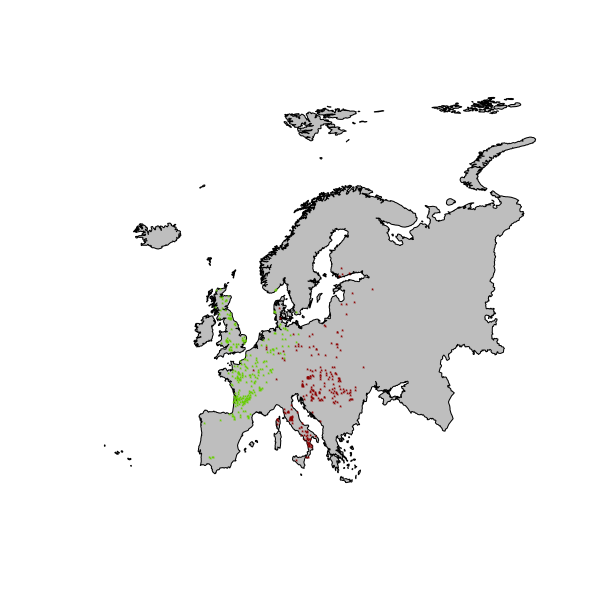
\includegraphics{mopa-mopa2}

\section{Environmental variables}

Predictor variables are typically organized as raster (grid) type files. The set of predictor variables (rasters) can be used to make a '\texttt{RasterStack}', which is a collection of '\texttt{RasterLayer}' objects (see the \texttt{raster} package for more info) (http://www.cran.r-project.org/web/packages/dismo/vignettes/sdm.pdf)

\begin{Schunk}
\begin{Sinput}
> # RatserStack of envirinmental variables
> data(biostack)
> plot(biostack)
\end{Sinput}
\end{Schunk}
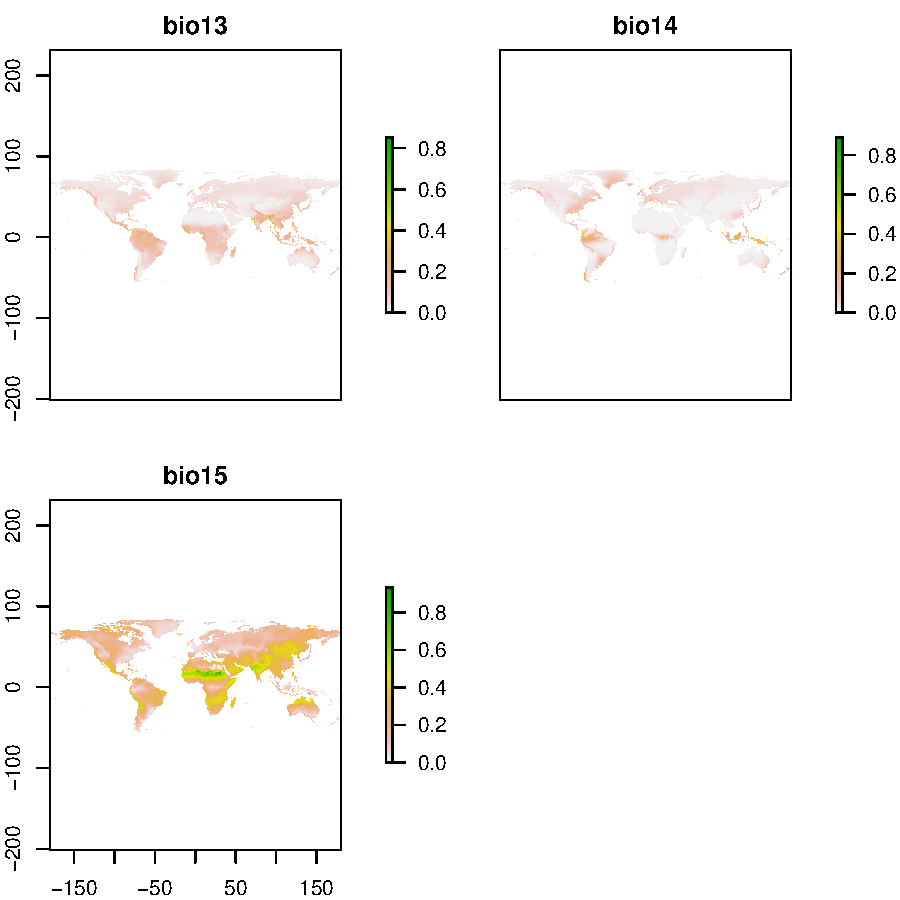
\includegraphics{mopa-mopa3}

\chapter{Study area and background}

\section{Creation of the background grid}

The regular point grid which covers the continental area can be created as follows:

\begin{Schunk}
\begin{Sinput}
> library(raster)
> ac<-xyFromCell(biostack[[1]],  1:ncell(biostack[[1]]))
> ex<-extract(biostack[[1]], ac)
> sp_grid<-SpatialPoints(ac[-which(is.na(ex)),])
> projection(sp_grid)<-CRS("+proj=longlat +init=epsg:4326")
\end{Sinput}
\end{Schunk}

\section{Limit study area to the bounding boxes around presences}

\begin{Schunk}
\begin{Sinput}
>  oak.extension<-boundingCoords(Oak_phylo2)
\end{Sinput}
\end{Schunk}

Intersection of the background point grid with the bounding boxes. A list with two objects is obtained, (1) bbs: polygon shape of the bounding boxes and (2) bbs.grid: list of data frames of the background point grid limited by the bounding coordinates.


\begin{Schunk}
\begin{Sinput}
> box.grid<-delimit(oak.extension, sp_grid, names(Oak_phylo2))
> plot(box.grid[[1]])
> for (i in 1:length(Oak_phylo2)){
+   points(Oak_phylo2[[i]], col=colors()[i*50])
+ }
\end{Sinput}
\end{Schunk}
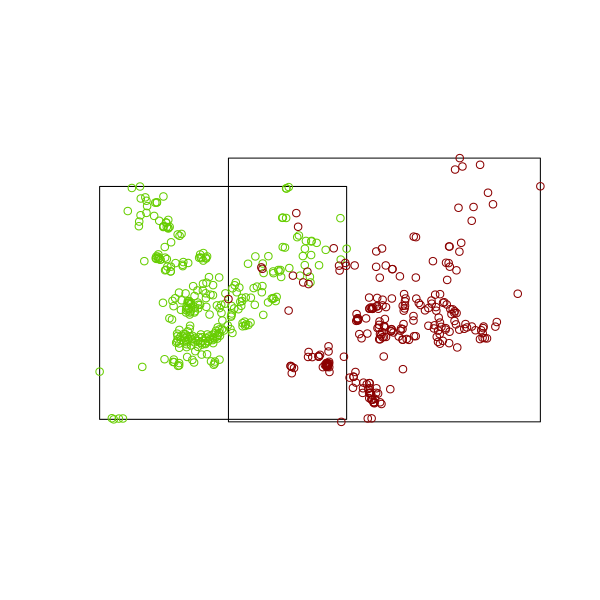
\includegraphics{mopa-mopa6}


\chapter{Three--step pseudo--absences generation}

 
\section{STEP1: environmental profiling}

\begin{Schunk}
\begin{Sinput}
> unsuitable.bg <-OCSVMprofiling(xy = Oak_phylo2, 
+                     varstack = biostack, 
+                     bbs.grid = box.grid$bbs.grid)
> plot(unsuitable.bg$absence$H11, pch="*")
> points(unsuitable.bg$presence$H11, pch="*", col= "pink2")
\end{Sinput}
\end{Schunk}
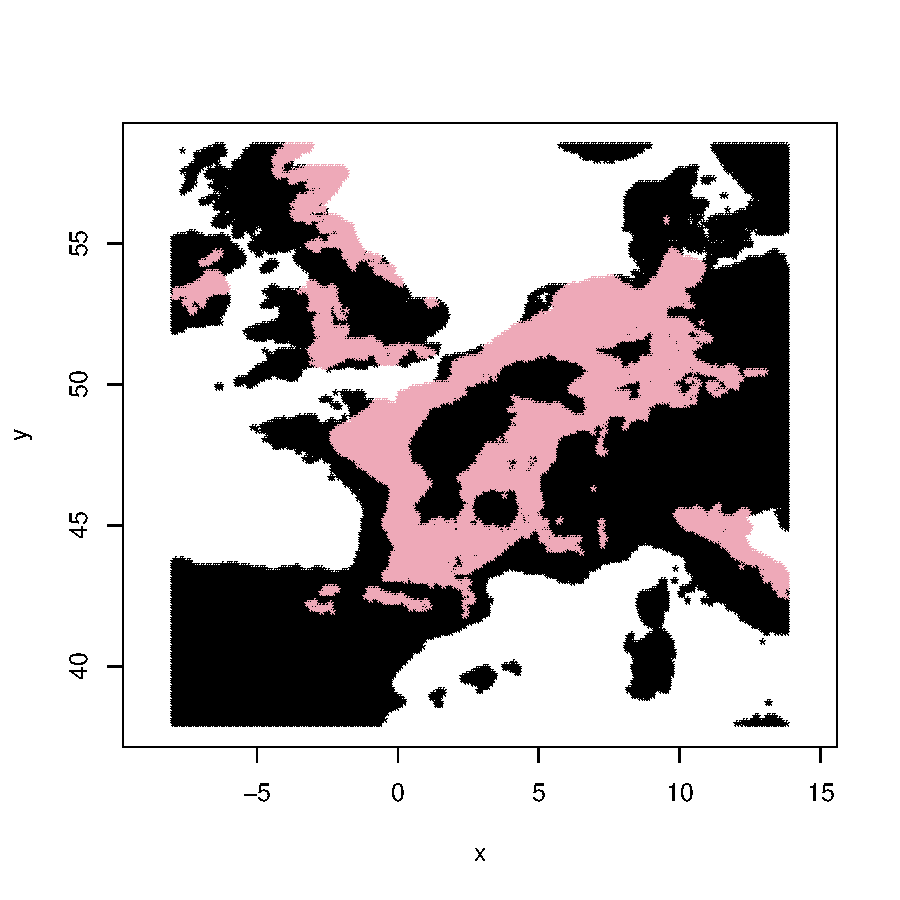
\includegraphics{mopa-mopa7}


\section{STEP2: background extents}

Sequence of 100 km between distances, from 20 km to the length of the half diagonal of the bounding box:

\begin{Schunk}
\begin{Sinput}
> ext <-bgRadio(xy = Oak_phylo2, bounding.coords = oak.extension, 
+ 	bg.absence = unsuitable.bg$absence, start = 0.166,
+   by = 0.83, unit = "decimal degrees")
\end{Sinput}
\begin{Soutput}
[1] "creating background point-grids for species 1 out of 2"
[1] "creating background point-grids for species 2 out of 2"
\end{Soutput}
\begin{Sinput}
> plot(ext$H11$km520, col="green4", pch="*")
> points(ext$H11$km120, pch="*")
> points(ext$H11$km20, pch="*", col="blue")
> points(Oak_phylo2$H11, col="red", pch= ".", cex=1.5)
\end{Sinput}
\end{Schunk}
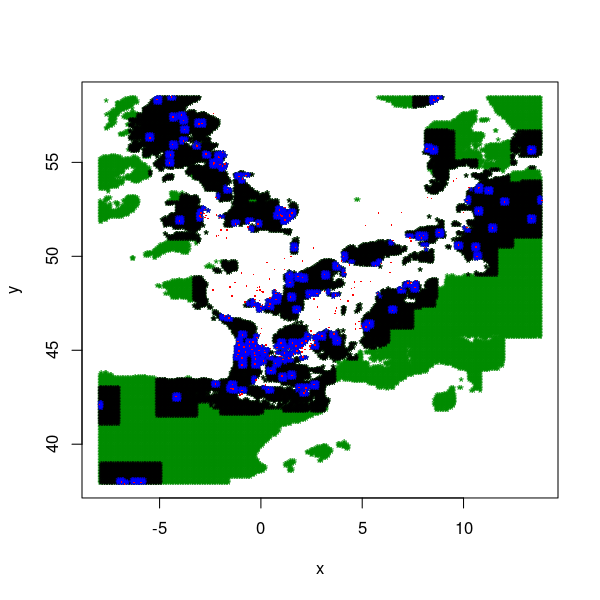
\includegraphics{mopa-mopa8}

\section{STEP3: pseudo--absences sampling}

\subsection{At random}

\begin{Schunk}
\begin{Sinput}
> pa_random <-PseudoAbsences(xy = Oak_phylo2, bg.grids = ext, 
+ 	exclusion.buffer = 0.0083, prevalence = 0.5, 
+   kmeans = FALSE)
\end{Sinput}
\begin{Soutput}
[1] "generating pseudo-absences for species 1 out of 2"
[1] "generating pseudo-absences for species 2 out of 2"
\end{Soutput}
\begin{Sinput}
> plot(ext$H11[[5]], pch="*", col= "grey", cex=.5)
> points(pa_random$H11[[5]], col="red", pch=".", cex=4)
> points(Oak_phylo2$H11, col="blue", pch=".", cex=3)
> 
\end{Sinput}
\end{Schunk}
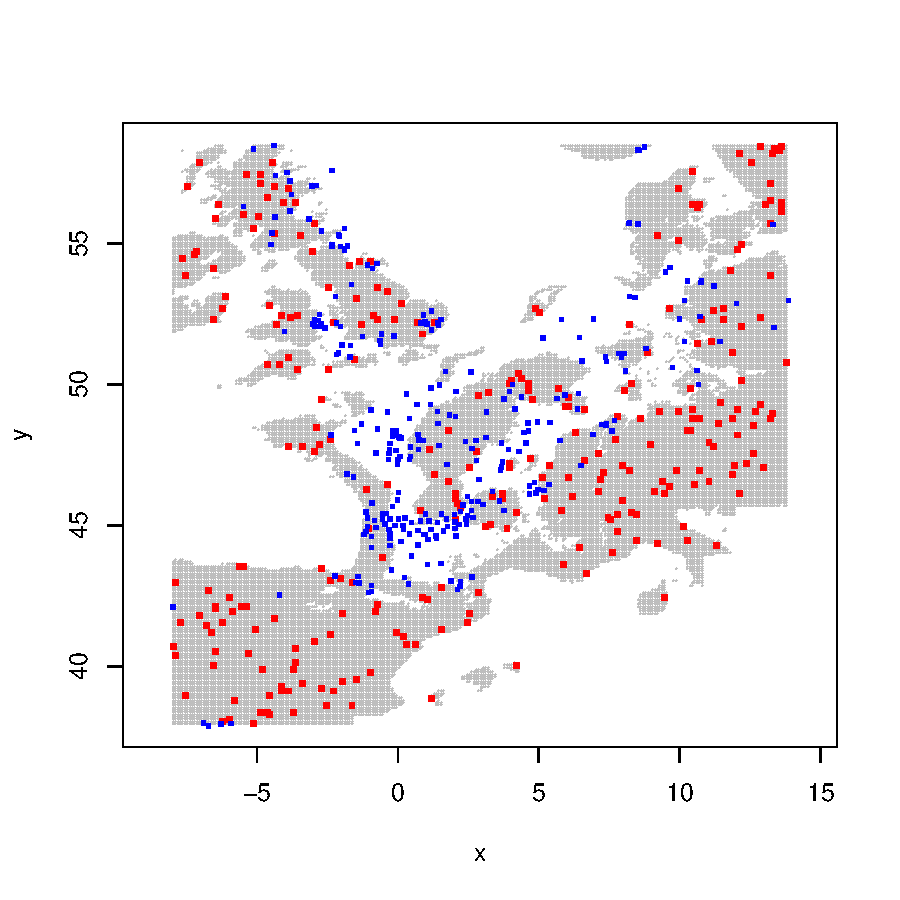
\includegraphics{mopa-mopa9}

\subsection{With k--means clustering}

\begin{Schunk}
\begin{Sinput}
> pa_kmeans <-PseudoAbsences(xy = Oak_phylo2, bg.grids = ext, 
+ 	exclusion.buffer = 0.0083, prevalence = 0.5, 
+   kmeans = TRUE)
\end{Sinput}
\begin{Soutput}
[1] "generating pseudo-absences for species 1 out of 2"
[1] "generating pseudo-absences for species 2 out of 2"
\end{Soutput}
\begin{Sinput}
> plot(ext$H11[[5]], pch="*", col= "grey", cex=.5)
> points(pa_kmeans$H11[[5]], col="red", pch=".", cex=4)
> points(Oak_phylo2$H11, col="blue", pch=".", cex=3)
\end{Sinput}
\end{Schunk}
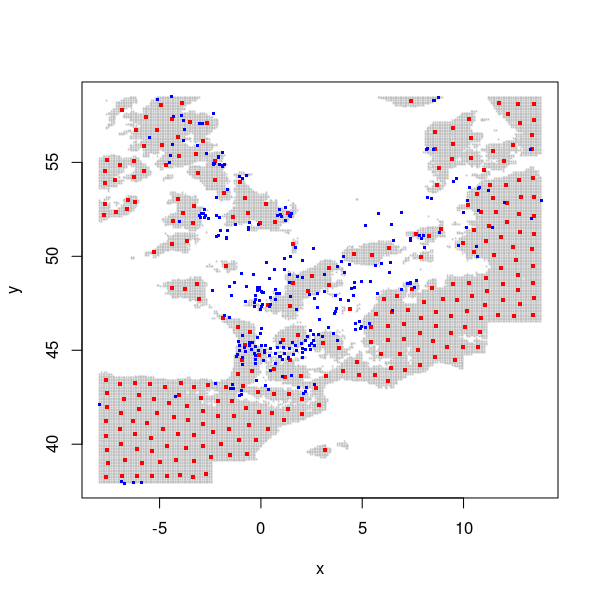
\includegraphics{mopa-mopa10}

\section{Put presences and pseudo--absences together}

\begin{Schunk}
\begin{Sinput}
> presaus <-bindPresAbs(presences = Oak_phylo2, 
+                       absences = pa_random)
\end{Sinput}
\end{Schunk}


\chapter{Species distribution modeling}


The \texttt{allModeling} function.Modelling and cross validation. Algorithms supported are "glm", "svm", "maxent", "mars", "randomForest", "cart.rpart" and "cart.tree"

\begin{Schunk}
\begin{Sinput}
> modirs <-allModeling(data = presaus, varstack = biostack, 
+               k = 10, algorithm = "mars", destdir = getwd(), 
+               projection = CRS("+proj=longlat +init=epsg:4326"))
\end{Sinput}
\end{Schunk}

Named Rdata objects are stored in the specified path. Each Object is given the a name indicating the algorithm, background extent, and species in this order (if a single species is provided no name is given for de species). Character object with listed files is returned. Each Rdata consists of a list with six components:

	1.-allmod: fitted model with all data for training 
	2.-auc: AUC statistic in the cross validation
	3.-kappa: kappa statistic in the cross validation
	4.-tss: true skill statistic in the cross validation
	5.-mod: fitted model with partitioned data 
	6.-p: cross model prediction 


To selected the model corresponding to the geographical extent beyond which the AUC scored by the model does not increase we need to load the generated data and extract auc values.

\begin{Schunk}
\begin{Sinput}
> auc_mars <-loadTestValues(data = presaus, test = "auc", 
+                           algorithm = "mars")
\end{Sinput}
\begin{Soutput}
[1] "loading values for species 1"
[1] "loading values for species 2"
\end{Soutput}
\begin{Sinput}
> library(lattice)
> levelplot(auc_mars ,aspect=5 ,at =seq(0.5,1,0.01), 
+           col.regions=bpy.colors, xlab="Haplogroups", 
+           ylab="Background extent (km)", main = "AUC")
\end{Sinput}
\end{Schunk}
\includegraphics{mopa-mopa13}

To extract the extent at which maximum AUC values is scored:

\begin{Schunk}
\begin{Sinput}
> ind<-indextent(auc_mars)
> ind
\end{Sinput}
\begin{Soutput}
km1220 km1120 
    13     12 
\end{Soutput}
\end{Schunk}

Thus, the \texttt{ind} object in this example gives the index of the background extent to be considered for each group/species and is going to be used to extract definitive model components and data. For example:

\begin{Schunk}
\begin{Sinput}
> def <-loadDefinitiveModel(presaus, ind, "allmod", "mars")
> #example of prediction
> projectionland <-biomat(cbind(box.grid[[2]][[1]], 
+                     rep(1,nrow(box.grid[[2]][[1]]))), 
+                     biostack)
> p <-predict(def[[1]], projectionland[,-1])->p
> spp<-SpatialPixelsDataFrame(box.grid[[2]][[1]], 
+                             as.data.frame(p))
> ras<-raster(spp)
> plot(ras)
\end{Sinput}
\end{Schunk}
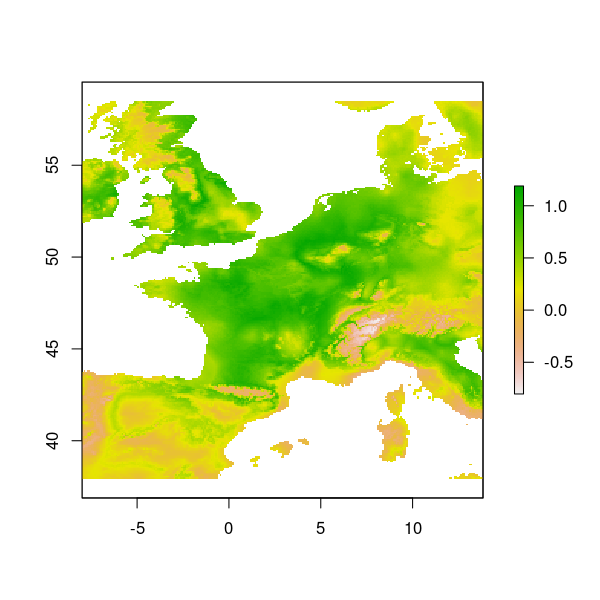
\includegraphics{mopa-mopa15}




%unsrtnat
\bibliographystyle{plainnat}
\bibliography{gen}



\end{document}


